\documentclass[11pt,a4paper]{article}
\usepackage{physics, amsmath,amsfonts,amsthm,amssymb, mathtools,steinmetz, gensymb, siunitx}	
\usepackage{bm}
\usepackage[top=42pt,bottom=42pt,left=70pt,right=70pt]{geometry}  % to make pages wider
\usepackage{setspace}
\usepackage{caption}
\usepackage{tikz}
\usepackage{pgf,tikz,pgfplots,wrapfig}
\usepackage{mathrsfs}
\usepackage{fancyhdr}
\usepackage{float}
\usepackage{array}
\usepackage{unicode-math}
\usepackage{booktabs,multirow}

\usepackage{graphicx}  % need this for figures etc.
\usepackage{url}  % to handle urls 
\usepackage[comma,authoryear]{natbib}  % for authordate ref style --  allows \citet (textual), and \citep (parenthesized)
\usepackage[hidelinks]{hyperref}
%\hypersetup{colorlinks,citecolor=MidnightBlue, linkcolor=Navy}
%\hypersetup{allcolors=[rgb]{0.6, 0, 0},colorlinks=true}
\hypersetup{allcolors=[rgb]{0, 0, 0.33},colorlinks=true}

\usetikzlibrary{decorations.text, calc}
\pgfplotsset{compat=1.7}

\usetikzlibrary{decorations.pathreplacing,decorations.markings}
\usepgfplotslibrary{fillbetween}

\renewcommand {\cite} {\citep}  % default for cite is citet in natbib - so change it
\renewcommand\bibname{References}    % if not using newrucsthesis sty file
%\usepackage[style= ACM-Reference-Format, maxbibnames=6, minnames=1,maxnames = 1]{biblatex}
%\addbibresource{references.bib}

\newcommand{\vect}[1]{\boldsymbol{#1}}

\title{
\textsc{Literature Review of the Tracking and Detection of Human Facial Features and project revision}
}
\author{\textsc{J L Gouws}
\\Supervisor: \textsc{Mr. J Connan}
\\ \emph{Computer Science Department, Rhodes University}}
\date{\today
\\[1cm]}

\begin{document}

\maketitle

%In some sections you have to make a best guess (hypothesis), since you haven't done your MSc yet. 
\begin{abstract}
  Tracking objects in video streams is a powerful tool in computer vision.
  This research will investigate the recognition and tracking of multiple faces in settings where the faces are concurrently visible.
  The study will implement a tracking system that after, initialising with minimal input data, detects faces and tracks their motion in a video stream.
  The task of tracking starts by initialising the tracker with bounding boxes that define the faces of the targets in images. 
  %TODO fix these sentences
  The initialised tracker will be able to detect if a target face is present in or absent from an arbitrary video stream.
  The tracker will identify any visible target and follow its motion. 
  %TODO fix these sentences
  If a target face disappears and later reappears in the video stream, the tracker will be able to identify and track it again, provided the target remains in the field of view.
\end{abstract}

\newpage
\section{Introduction}
  Analysis of videos of crowds of people has many practical applications.
  Most real world situations that involve people have people that are moving.
  On top of that most often people are not isolated, but instead form groups of people.

  For these reasons it makes sense to investigate ways to develop a system that can efficiently and accurately detect and track multiple people in a video stream.
  Tracking targets in a video stream is by and large an understudied field.
  The literature is relatively limited in comparison with the number of real world applications of tracking systems.

%\input{researchstatement}
%\input{researchobjectives}
%\section{Related Works}\label{sec:relatedWorks}
In 2011 \citeauthor{Kalal2011} invented the Tracking, Learning and Detection(TLD) framework for the longterm tracking of objects in a video stream.
Kalal's original implementation uses a median flow tracker, P-N learning, and a random forrest and nearest neighbour based detector \cite{KalalPHD}.
These three components give the respective tracking, learning and detection components of the system.

The learning compenent of TLD forms the backbone of the system, governing the interaction between the detector and tracker.
The three components exchange information as shown in Figure~\ref{fig:tld}, this allows the tracker to improve it's performance as time progresses \cite{Kalal2011}.
For the system to operate, it requires online learning--learning as data becomes available. 
Kalal developed the P-N Learning paradigm \cite{PNLearning}, a semi-supervised bootstrapping model \cite{murphy2012}, tailored to the needs of TLD.

\begin{figure}[!ht]
  \centering
   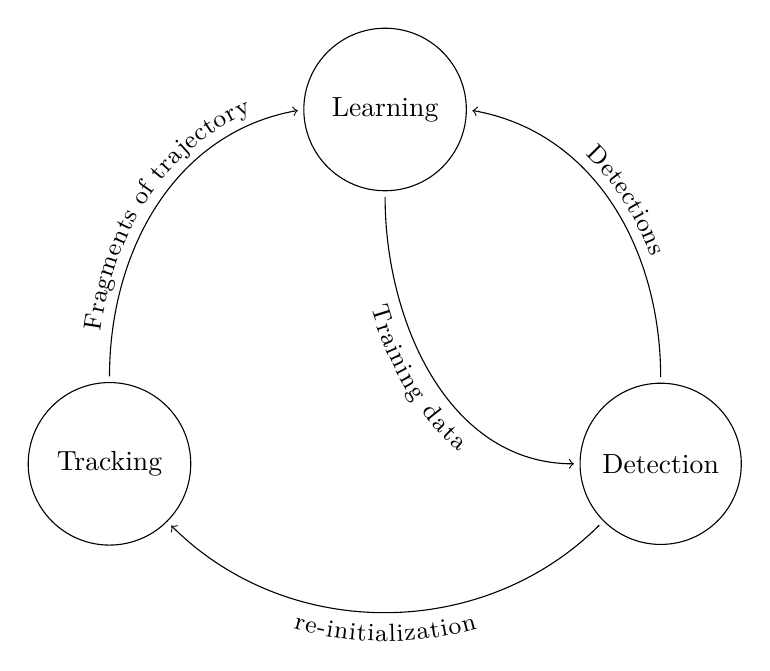
\begin{tikzpicture}[approach/.style={draw,very thick, fill=white, text width=5em,
         text centered, minimum height=2em,rounded corners=3ex, scale=0.1, everynode/.style={scale=0.1}},
         idea/.style={draw=black, circle,text width=5em,
            text centered, minimum height=2.5em},
         connections/.style={->,draw=black,shorten <=2pt,shorten >=2pt},
         reverseConnections/.style={<-,draw=black,shorten <=2pt,shorten >=2pt},
      ]

      \node[draw] at (0,0) (tracking) [idea]  {Tracking};
      \node[draw] at (3.5,4.5) (learning) [idea]  {Learning};
      \draw[connections, postaction={decorate, decoration={raise=1ex, text along path, text align=center, text={|\small|Fragments of trajectory}}}] (tracking.north)to[out=90,in=190] (learning.west) ;
      \node[draw] at (7,0) (detection) [idea]  {Detection};
      \draw[connections, postaction={decorate, decoration={raise=-2.5ex, text along path, text align=center, text={|\small|Training data}}}] (learning.south) to[out=270,in=180] (detection.west) ;
      \draw[reverseConnections, postaction={decorate, decoration={raise=1ex, text along path, text align=center, text={|\small|Detections}}}] (learning.east) to[out=350,in=90] (detection.north) ;
      \draw[reverseConnections, postaction={decorate, decoration={raise=-2.5ex, text along path, text align=center, text={|\small|re-initialization}}}] (tracking.south east) to[out=-45,in=225] (detection.south west) ;
   \end{tikzpicture}
   \caption{The interaction between tracking, learning and detection in TLD. Figure from \cite{Kalal2011}}
   \label{fig:tld}
\end{figure}

\citeauthor{Enriques2014} \cite{Enriques2014} propose Kernelized Correlation Filters(KCF) and the novel Dual Correlaion filter(DCF).
Both KCF and DCF use circulant matrices and the kernel Trick.
The implementation of KCF by \citeauthor{Enriques2014} uses a Gaussian Kernel, whereas the DCF implementation uses a linear kernel.
The calculations involved with the linear kernel are less computationally complex than KCF. 
DCF can, hence, be processed faster, but, at the cost of some tracking precision.

Work by \citeauthor{multichannelCorrFilters} \cite{multichannelCorrFilters} allows KCF and DCF to be applied to modern and useful feature descriptors.
\citeauthor{Enriques2014} show that KCF and DCF be be applied to Histogram of Oriented Gradient(HOG) features to track and detect objects in a video stream with lower computation times and better accuracy.
KCF and DCF applied to HOG features are shown to outperfrom many tracking systems Table~\ref{tab:trackers}.
The results shown by Table~\ref{tab:trackers} are obtained from running the algorithms on a standard four core desktop processor from \citedate{Enriques2014}.

\begin{table}
  \centering
  \begin{tabular}[t]{cccc}
    \toprule
    Algorithm & feature & Mean precision & Mean FPS \\
    \midrule
    KCF       & HOG     & 73.2\%         & 172      \\
    \hline
    DCF       & HOG     & 72.8\%         & 292      \\
    \hline
    KCF       & Raw pixels & 56.0\%      & 154      \\
    \hline
    DCF       & Raw pixels & 45.1\%      & 278      \\
    \midrule
    \midrule
    \multicolumn{2}{c}{TLD}   & 60.8\%      &  28      \\
    \hline
    \multicolumn{2}{c}{Struck\cite{struck}}& 65.6\%     &  20     \\
    \hline
    \multicolumn{2}{c}{MOSSE\cite{mosse}}& 43.1\%      &  615     \\
    \bottomrule
  \end{tabular}
  \caption{Comparison of various trackers, adapted from \cite{Enriques2014}}
  \label{tab:trackers}
\end{table}

The system implemented by \citeauthor{Enriques2014} does not, however, encorporate a failure recovery mechanism--section 8 of \cite{Enriques2014}.
In other words \citeauthor{Enriques2014} only explore KCF in the domain of ST.
This is in contrast to the original TLD system which provides a failure recovery mechanism in the detection component \cite{Kalal2011}.
The ST using KCF and DCF done by \citeauthor{Enriques2014} can be used in a TLD framework for LT.

\citeauthor{Ma2015Correlation} \cite{Ma2015Correlation} investigate the problem of single object LT using correlation tracking.
\citeauthor{Ma2015Correlation} use two Gaussian ridge regression \cite{murphy2012} models for tracking.
One model uses the relative change in background and target as time progresses, the other model tracks by using the target's appearance.
The first model is used to track the object's trajectory through fast motion and occlusions, and the second is used for scale change.
Using both tracking models they train an online detector that is both flexible(from first tracker model) and stable(from second tracker model).

\citeauthor{Ma2015Correlation} train a random fern classifier \cite{ferns2007} \cite{Kalal2011} online in order to handle tracker failure.
This solves the LT problem in a similar way to \citeauthor{KalalPHD}.

The Visual Object Tracking Challenge(VOT) is a challenge that benchmarks various trackers every year \cite{VOT2017} \cite{VOT2020}.
VOT investigates both ST and LT.
In recent years, VOT has also introduced a real time challenge \cite{VOT2020}.

There has also been investigation into the use of Convolutional Neural Networks in tracking \cite{CNNTracking}.
The work by \citeauthor{CNNTracking} offers high performance tracking of generic objects.
The system implemented by \citeauthor{CNNTracking} requires a large amount of offline training.

\citeauthor{onlineRL} \cite{onlineRL} propose a new online reinforcement learning method that can be used to train models with minimal input data.
\citeauthor{onlineRL} describe the \textit{Reanalyse} algorithm.
Given a state of a machine learning model the \textit{Reanalyse} algorithm generates training targets for the model from some input data.
When the model has improved by training, the \textit{Reanalyse} algorithm generates more training targets based on the new state of the model, the already seen input data, and any new input data.
The algorithm allows the available training data to be cycled--this allows the algorithm to extract most of the information from a limited dataset.

%\section{Approach to Research}
  Initially I will start by reading literature on tracking and facial recognition.
  This will mainly start by reviewing Kalal's work in TLD, namely his Doctoral thesis \cite{KalalPHD}.

  Next I will go into a phase of re-implementing predator in C++, with help from the OpenCV libraries.
  Once this is stable and running with decent performance, I will move onto the next stage.

  Next I will be looking at ways to improve my implementation of the TLD system.
  I will mainly focus on looking at improving the tracking and detection stages of the system.
  I will then spend a small amount of time looking at the learning component, but do not intend to completely change it.

  Next I will extend the tracking and detection system so that it is able to identify and track multiple targets in a video stream.
  This will probably require a lot of work and testing.
  It is important that the system is both reasonably accurate.
  It is particularly that the system does not get confused and misidentify objects in the start up phase.
  There is always high potential for confusion in the start up of system, where there are potentially similar looking faces.

  Finally I will be looking at ways to enhance the performance of tracking multiple objects.
  This will come later and mainly be considered and extension.
  It would be useful to have the system run on mobile devices or micro-computers, with the potential to be extended to a distributed system.

\input{researchstatement}
\section{Facial Recognition}
  Facial recognition is a standard element of computer vision with numerous applications.
  The goal of facial recognition is to label a face that is present in an image.
  \subsection{Eigenfaces}
  \citet{eigenFacesRecog} describe how to use principal component analysis (PCA) to determine features for facial recognition.
  PCA is used to determine eigenvectors, referred to as ``eigenfaces", that form a basis for the faces of concern.
  PCA can decompose any face, from a given set, into a linear combination of basis vectors; this is equivalent to representing a vector in Euclidean space in an eigenvector basis.
  A facial recognition system can use the decomposition's components to identify faces.
  
  This usage of eigenfaces allows for a more compact representation of a face.
  PCA finds a set of features that account for the most significant variation in a given collection of faces.
  This method allows \citet{eigenFacesRecog} to achieve facial recognition that is ``fast, relatively simple, and has been shown to work well in a constrained environment \cite{eigenFacesRecog}.'' 

  \citet{ICAFaceRecog} suggest using Independent Component Analysis (ICA) instead of PCA.
  ICA is a generalisation of PCA that considers the relationship of distant pixels.
  This mechanism allows ICA to encode more information in the eigenvectors compared to PCA.

  A machine learning model can use this set of features to identify a given face.
  One option is to use a neural network which offers high accuracy and quick recognition \cite{eigenFacesRecog, ICAFaceRecog}.
  Alternatively, a naive Bayes classifier which amenable to online learning \cite{murphy2012} can do the recognition.

  \subsection{Multi-Pose Face Recognition}
  In a realistic video stream it is atypical for all the faces to be facing the camera at a given time.
  The faces might change pose from frontal to profile.
  It is thus key for a detector to recognize faces that both from a frontal and portrait pose, if it is going to used on real world data.

  \citeauthor{viewBasedFaceRecog} \cite{viewBasedFaceRecog} suggest two solutions to the problem of Multi-Pose Face Recognition using eigenfaces.
  First, a single high dimensional eigenface space can be used.
  In this face-space a basis vector contains information about the face and its orientation.
  Second, different face-spaces can be used for different orientations.
  Each face-space is defined by using PCA on images of all the faces taken a given viewpoint, for example 10 degrees left of frontal view.

  \citeauthor{PoseFaceRec} \cite{PoseFaceRec} describe ways to recognise and track a face that takes on multiple poses.
  The system proposed by \citeauthor{PoseFaceRec} has three components: Haar Cascades based face detection, weighted modular PCA based face recognition and Kalman tracker.
  


\section{Learning}
  Consider a continious video stream that is being analyzed by a pre-trained tracking system.
  This video stream is a constant flux of information, and some of the information might not have been encountered the tracking system's history.
  The information contained in the video stream can, thus, be used to improve the tracking system.
  Improving the system requires learning mechanisms, specifically online learning--learning where information becomes available while the system is in operation.
  \subsection{Online Learning}
  One option for solving the problem of online learning is Stochastic Gradient Descent.
  Stochastic gradient descent aims to minimize a cost function, $f(\mathbf{\theta})$, by changing the parameters, $\mathbf{\theta}$.
  The parameters are updated in sequential steps of the form:
  \begin{equation*}
    \mathbf{\theta}_{k + 1} = G(\mathbf{\theta}, f())
  \end{equation*}

  \subsection{Reinforcement Learning}
  \citet{onlineRL} propose a new online reinforcement learning method that can train models with minimal input data.
  In their paper, \citeauthor{onlineRL} describe the \textit{Reanalyse} algorithm.
  The \textit{Reanalyse} algorithm uses a machine learning model's state and input data from the environment to generate training targets for the model.
  When the model has improved by training, the \textit{Reanalyse} algorithm generates more training targets based on the new state of the model, the already seen input data, and any new input data.
  The algorithm cycles the available training data--this allows the algorithm to extract most of the information from a limited dataset.

  \subsection{Updating Template Trackers}
  Template tracking \cite{templateUpdate} assumes that the appearace of the target object does not undergo changes.
  The results in simplistic tracking and the tracker will fail if the target undergoes a change in orientation or a change of view.
  \citeauthor{templateUpdate} propose solutions to this, and discuss the problems around the solutions.
  The problems are a result of what is known as the stability-plasticity dilema \cite{grossberg1987}.

  Everytime a tracker template is updated, some error in the template is introduced.
  This causes the tracker to drift, and evetually cause the tracker to fail \cite{templateUpdate}.

  Suppose that $\mathbf{x}$ is the coordinate vector of a pixel in the $n^{\text{th}}$ frame $I_n(\mathbf{x})$ of a video.
  Let $T(\mathbf{x})$ be the template of the target image, and $T_n(\mathbf{x})$ be the template of the object in the $n^\text{th}$ frame of a video sequence.
  The warp of the image $\mathbf{W}(\mathbf{x};\mathbf{p})$ represents the allowed deformations of the template given a set of parameters $\mathbf{p}$ which define a deformation.
  The warp maps a pixel from the template frame to the coordinates of the video frame $I_n(\mathbf{x})$.

  Given these defintions, the problem of tracking formally reduces to computing the parameters for the deformation of the object:
  \begin{equation}
    \mathbf{p}_n = \arg \min_\mathbf{p} \sum_{\mathbf{x} \in T_n}\left[I_n(\mathbf{W}(\mathbf{x};\mathbf{p})) - T_n(\mathbf{x})\right]^2
    \label{eq:newTempParams}
  \end{equation}
  And then updating the tracking template based on the warp of the $n^\text{th}$ frame, for example a naive update is \cite{templateUpdate}:
  \begin{equation*}
    \forall n \geq 1, T_{n+1}(\mathbf{x}) = I_n(\mathbf{W}(\mathbf{x};\mathbf{p}_n))
  \end{equation*}

  Implementing this requires a gradient descent algorithm for non-linear optimizations.
  Equation \ref{eq:newTempParams} now becomes:
  \begin{equation}
    \mathbf{p}_n^* = \mathrm{gd} \min_{\mathbf{p} = \mathbf{p}_{n-1}} \sum_{\mathbf{x} \in T_n}\left[I_n(\mathbf{W}(\mathbf{x};\mathbf{p})) - T_n(\mathbf{x})\right]^2
    \label{eq:paramUpdate}
  \end{equation}
  With $\mathrm{gd} \min_{\mathbf{p}}$ indicating a gradient descent minimization starting from the warp parameters of the $(n-1)^\text{th}$ frame.
  
  Using Equation~\ref{eq:paramUpdate}, \citeauthor{templateUpdate} suggest a template update with drift correction given by:
  \begin{align*}
    &\text{If } \norm{\mathbf{p_n}^* - \mathbf{p_n}} \leq \varepsilon \text{ Then } T_{n+1} (\mathbf{x}) = I_n(\mathbf{W}(\mathbf{x};\mathbf{p}_n^*))\\
    &\text{else } T_{n+1}(\mathbf{x}) = T_n(\mathbf{x})
  \end{align*}
  Given some small threshold $\varepsilon > 0$.
  This updates the template if retaining the template would cause tracker drift, otherwise the template is not updated.

  \input{PNLearning}

\section{Tracking}
  Tracking is a versatile form of computer vision present in almost all forms of video analysis.
  The task of tracking is to determine the trajectory of an object in a video stream.
  
  \subsection{General Comparison of Trackers}
  The Visual Object Tracking Challenge(VOT) is a challenge that benchmarks various trackers every year \cite{VOT2017, VOT2020}.
  VOT investigates both ST and LT.
  VOT has also introduced a real-time challenge \cite{VOT2020}.

  In the VOT 2020 challenge, most trackers use deep features instead of handpicked features that were predominant in the past.
  In the short-term tracking challenge, 86 \% of trackers used deep features.
  Deep discriminative correlation filters (DCF) \cite{danelljan2019} have succeeded in many recent VOT challenges. 
  Of the short-term trackers in VOT2020, 15 used deep DCF.

  All of the long-term trackers in VOT 2020 used convolutional neural networks.
  Several long-term challenge trackers use MDNet \cite{CNNTracking} as a basis for object presence detection.
  One of the long-term trackers used deep DCF; Another used siamese convolutional neural networks.

  \input{CNN}
  \subsection{Tracking with Correlation Filters}
\citet{Enriques2014} propose Kernelized Correlation Filter(KCF) and the novel Dual Correlation Filter(DCF).
Both KCF and DCF use circulant matrices and the kernel trick.
The implementation of KCF by \citeauthor{Enriques2014} uses a Gaussian kernel, whereas the DCF implementation uses a linear kernel.
The calculations involved with the linear kernel are less computationally complex than for the Gaussian kernel. 
Therefore, DCF can be processed faster at the cost of some tracking precision.

Work by \citet{multichannelCorrFilters} allows KCF and DCF to exploit modern and useful feature descriptors.
\citeauthor{Enriques2014} show that KCF and DCF can be applied to the Histogram of Oriented Gradients (HOG) descriptor to track and detect objects in a video stream with lower computation times and better accuracy.
Table~\ref{tab:trackers} shows that KCF and DCF applied to HOG features outperform many tracking systems.
The results shown in Table~\ref{tab:trackers} give the tracker's performance on a standard four core desktop processor from 2014.

\begin{table}
  \centering
  \begin{tabular}[t]{cccc}
    \toprule
    Algorithm & feature & Mean precision & Mean FPS \\
    \midrule
    KCF       & HOG     & 73.2\%         & 172      \\
    \hline
    DCF       & HOG     & 72.8\%         & 292      \\
    \hline
    KCF       & Raw pixels & 56.0\%      & 154      \\
    \hline
    DCF       & Raw pixels & 45.1\%      & 278      \\
    \midrule
    \midrule
    \multicolumn{2}{c}{TLD}   & 60.8\%      &  28      \\
    \hline
    \multicolumn{2}{c}{Struck\cite{struck}}& 65.6\%     &  20     \\
    \hline
    \multicolumn{2}{c}{MOSSE\cite{mosse}}& 43.1\%      &  615     \\
    \bottomrule
  \end{tabular}
  \caption{Comparison of various trackers, adapted from \cite{Enriques2014}}
  \label{tab:trackers}
\end{table}

The system implemented by \citeauthor{Enriques2014} does not incorporate a failure recovery mechanism--section 8 of \cite{Enriques2014}.
In other words, \citeauthor{Enriques2014} only explore KCF in the domain of ST.
This approach contrasts the original TLD system that provides a failure recovery mechanism in the detection component \cite{Kalal2011}.
The TLD framework can employ \citeauthor{Enriques2014}s' short-term KCF or DCF tracking system  to build a long-term tracker.

\citet{Ma2015Correlation} investigate the problem of single object LT using correlation tracking.
\citeauthor{Ma2015Correlation} use two Gaussian ridge regression \cite{murphy2012} models for tracking.
One model uses the relative change in background and target as time progresses; the other model tracks by using the target's appearance.
The first model tracks the object's trajectory through fast motion and occlusions, and the second tracks scale changes.
Using both tracking models, they train an online detector that is both flexible(from the first tracker model) and stable(from the second tracker model).

\citeauthor{Ma2015Correlation} train a random fern classifier \cite{ferns2007, Kalal2011} online to handle tracker failure.
This solution for long-term tracking is similar to what \citeauthor{KalalPHD} does with TLD.

  \subsection{Tracking, Learning, Detection}\label{sec:tld}

  \begin{figure}[!ht]
    \centering
     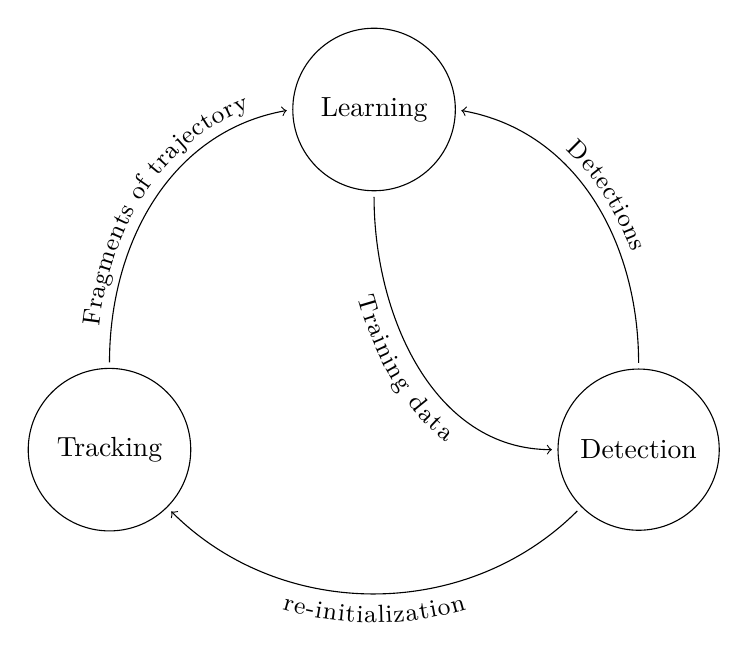
\begin{tikzpicture}[approach/.style={draw,very thick, fill=white, text width=5em,
           text centered, minimum height=2em,rounded corners=3ex},
           idea/.style={draw=black, circle,text width=5em,
              text centered, minimum height=2.5em},
           connections/.style={->,draw=black,shorten <=2pt,shorten >=2pt},
           reverseConnections/.style={<-,draw=black,shorten <=2pt,shorten >=2pt},
           scale=0.96, everynode/.style={scale = 0.96},
        ]

        \node[draw] at (0,0) (tracking) [idea]  {Tracking};
        \node[draw] at (3.5,4.5) (learning) [idea]  {Learning};
        \draw[connections, postaction={decorate, decoration={raise=1ex, text along path, text align=center, text={|\small|Fragments of trajectory}}}] (tracking.north)to[out=90,in=190] (learning.west) ;
        \node[draw] at (7,0) (detection) [idea]  {Detection};
        \draw[connections, postaction={decorate, decoration={raise=-2.5ex, text along path, text align=center, text={|\small|Training data}}}] (learning.south) to[out=270,in=180] (detection.west) ;
        \draw[reverseConnections, postaction={decorate, decoration={raise=1ex, text along path, text align=center, text={|\small|Detections}}}] (learning.east) to[out=350,in=90] (detection.north) ;
        \draw[reverseConnections, postaction={decorate, decoration={raise=-2.5ex, text along path, text align=center, text={|\small|re-initialization}}}] (tracking.south east) to[out=-45,in=225] (detection.south west) ;
     \end{tikzpicture}
     \caption{The interaction between tracking, learning and detection in TLD. Figure from \cite{Kalal2011}}
     \label{fig:tld}
  \end{figure}

  In 2011 \citeauthor{Kalal2011} invented the Tracking, Learning and Detection(TLD) framework for the longterm tracking of objects in a video stream.
  Kalal's original implementation uses a median flow tracker, P-N learning, and a random forrest and nearest neighbour based detector \cite{KalalPHD}.
  These three components give the respective tracking, learning and detection components of the system.

  The learning compenent of TLD forms the backbone of the system, governing the interaction between the detector and tracker.
  The three components exchange information as shown in Figure~\ref{fig:tld}, this allows the tracker to improve it's performance as time progresses \cite{Kalal2011}.
  By the nature of TLD, online learning is required for the learning component.
  Kalal developed the P-N Learning paradigm \cite{PNLearning}, a semi-supervised bootstrapping model \cite{murphy2012}, tailored to the needs of TLD.

  The tracker of TLD outputs a bounding box for the target object in every frame.
  A second bounding box for the target object is also produced by the detector.
  The P-experts and N-experts of the learning component use these bounding boxes to determine the false positives and the false negatives of the detector.
  This is used to update the detector, as descibed in Section \ref{sec:pnlearning}.
  An integrator is then used to combine the bounding boxes given by the tracker and detector \cite{Kalal2011}.


\section{Methodology}
\usetikzlibrary{shapes.geometric, arrows}

\tikzstyle{startstop} = [rectangle, rounded corners, minimum width=3cm, minimum height=1cm,text centered, draw=black]
\tikzstyle{io} = [trapezium, trapezium left angle=70, trapezium right angle=110, minimum width=3cm, minimum height=1cm, text centered, draw=black]
\tikzstyle{process} = [rectangle, minimum width=3cm, minimum height=1cm, text centered, draw=black]
\tikzstyle{decision} = [diamond, aspect = 2.5,minimum width=2cm, minimum height=0.5cm, text centered, draw=black]
\tikzstyle{arrow} = [thick,->,>=stealth]
\tikzstyle{line} = [thick]

\subsection{Methodology Overview}
\begin{figure}[H]
  \centering
  \begin{tikzpicture}[node distance=2cm]
    \node (proposal) [startstop] {Proposal};
    \node (litRev) [io, below of=proposal] {Review Literature};
    \node (data) [io, below of=litRev] {Obtain public data};
    \node (partImp) [process, below of=data] {Partial Implementation};
    \node (testImp) [process, below of=partImp] {Test Implementation};
    \node (passTest) [decision, below of=testImp, yshift=-1cm, text width = 17em, inner sep = -0.8em] {Satisfactory Performance and insufficient time};
    \node (thesis) [startstop, below of=passTest, text width = 17em, yshift=-0.8cm] {Finish Thesis};
    \coordinate [right of=passTest, xshift = 10em] (failTest);
    \coordinate [right of=partImp, xshift = 10em] (reImp);
    \node (reLit) [io, inner sep = 0.8em] at ($(reImp)!0.5!(failTest)$) {Review more literature};

    \draw[arrow] (proposal) -- (litRev);
    \draw[arrow] (litRev) -- (data);
    \draw[arrow] (data) -- (partImp);
    \draw[arrow] (partImp) -- (testImp);
    \draw[arrow] (testImp) -- (passTest);
    \draw[arrow] (passTest) -- node[anchor = east] {Yes} (thesis);
    \draw[line] (passTest) -- node[anchor = south] {No} (failTest);
    \draw[line] (reImp) -- (partImp);
    \draw[line] (reImp) -- (reLit) -- (failTest);
  \end{tikzpicture}
  \caption{Conceptual overview of design methodology}
\end{figure}

\section{Approach to Research}
  Initially I will start by reading literature on tracking and facial recognition.
  This will mainly start by reviewing Kalal's work in TLD, namely his Doctoral thesis \cite{KalalPHD}.

  Next I will go into a phase of re-implementing predator in C++, with help from the OpenCV libraries.
  Once this is stable and running with decent performance, I will move onto the next stage.

  Next I will be looking at ways to improve my implementation of the TLD system.
  I will mainly focus on looking at improving the tracking and detection stages of the system.
  I will then spend a small amount of time looking at the learning component, but do not intend to completely change it.

  Next I will extend the tracking and detection system so that it is able to identify and track multiple targets in a video stream.
  This will probably require a lot of work and testing.
  It is important that the system is both reasonably accurate.
  It is particularly that the system does not get confused and misidentify objects in the start up phase.
  There is always high potential for confusion in the start up of system, where there are potentially similar looking faces.

  Finally I will be looking at ways to enhance the performance of tracking multiple objects.
  This will come later and mainly be considered and extension.
  It would be useful to have the system run on mobile devices or micro-computers, with the potential to be extended to a distributed system.

\subsection{Timeline}
The timeline for this project has been revised since the Proposal version.
Most of the implementation deadlines now fall in the June and July Holiday, this is on account of exams and busy term times.
\begin{center}
  \begin{tabular}{l l}
    \toprule
      Time & Deliverable\\
    \midrule
      30 March 2022     & Seminar 1: Presentation of project\\
      11 April 2022     & Draft proposal\\
      19 April 2022     & Final proposal\\
      6 May 2022        & Literature review\\
      20 May 2022       & Obtaining suitable public videos\\
      28 May 2022       & Functional re-implementation of TLD\\
      28 June 2022      & Using KCF as Tracking stage of tracker\\
      30 June 2022      & Implementing DCF and comparing to KCF\\
      6 July 2022       & Reviewing VOT for better trackers\\
      11 July 2022      & Investingating random fern detectors\\
      11-13 July 2022   & Seminar 2: Progress Presentation\\
      25 July 2022      & Final decision on Tracking and Detection stages.\\
      12 August 2022    & Extension of system to multiple targets\\
      19 August 2022    & Progress Report\\
      26 August 2022    & Test and make small improvements the system\\
      3 October 2022    & First Draft of thesis\\
      10 Octorber 2022  & Completion of implementation\\
      14 October 2022   & Short ACM-style paper\\
      17-19 October 2022& Seminar 3: Final Oral presentation\\
      28 October 2022   & Final project submission\\
    \bottomrule
  \end{tabular}
\end{center}


%\section{Limitations}
  The first concern of this research is in regards to ethics.
  Owing to ethical concerns, the system can only be tested on public data, which limits the test cases for the system.
  An ethical clearance is required to test the system on examples that are closer to real world applications.
  Time restrictions on the project make doing an ethical clearance impractical.

  Further on this point, the second limitation of this research is time.
  The project is set to take one year, being an honours project.
  There is only so much literature that can be reviewed and still allow for the implementation of a system.
  On account of this restiction, the research might not explore certain areas of concern.

  This research is only concerned with the tracking of faces.
  There are many other features that can be used to detect and track humans, for example gait. 
  Sometimes, there are also needs to track objects other than faces. 
  The system implemented by the research cannot guarantee tracking capabilities of objects other than human faces.

  There will be an upper limit on the number of faces that can be tracked simultaneously in real time.
  There are two problematic cases: First, limited compute power, second screen space.
  The first case occurs if the runtime complexity of the implemented system increases proportionally to the number of faces being tracked.
  Formally, if system has runtime complexity worse than $O(1)$, the system will eventually fail to track, in real time, as more faces are added.
  The second problem case occurs in very large, dense crowds of faces where there is not enough space in the field of view for all the faces, or some faces are captured in insufficient resolution.

%\section{Applications}
  This reaseach has multiple real world applications.
  One includes an automated class register that can be used in schools or for university lecture attendance.

  Another application on the larger scale is a security system for monitoring the motion of people.
  This application requires the system to be extended to a distributed system.
  This could enhance airport security for example, adding functionality to label suspected terrorists.

  The system also has potential to be used as an assistive technology for visually impaired people.
  If the system can be ported to a mobile device, it could help a visually impaired person identify people at a party or on a television program.
  This application assumes the system has had the appropriate offline training in it's initialization phase.

\section{Conclusion}
  \subsection{Conclusion of the Literature Review}
    The Visual Object Tracking Challenge(VOT) ranks many current tracking systems every year \cite{VOT2017, Kristan2020a}.
    The challenge ranks trackers in different categories, the two main categories are long-term and short-term tracking.
    VOT ranks the trackers based on various metrics that indicate the accuracy of the tracker. 
    VOT does not, however, require trackers to run at real-time frame rates, some trackers run at less than one frame a second.

    There are, at present, two main approaches to solve the problem of long-term tracking in real time.
    The first approach uses correlation tracking and training a classifier online \cite{Ma2015Correlation, Enriques2014, Kalal2011}.
    These methods require little set-up time, and can track single unkown objects in a video stream.

    The second approach uses CNNs \cite{bertinetto2016}.
    This approach requires an offline training stage, but the offline training stage need not be repeated.
    CNNs allow for high accuracy tracking \cite{CNNTracking, bertinetto2016}, and provided that online learning is not required, the trackers can process videos at high frame rates \cite{Kristan2020a}.

    From a user's point of view, the operation of the CNN approach and the correlation approach seem identical.
    After the CNN has undergone offline learning, the CNN tracking systems only require a single image with a bounding box to track an unkown object.

\subsection{Revised Project Conclusion}
This research uses the Tracking, Learning and Detection(TLD) framework to implement a system that can simultaneously track and detect multiple faces.
TLD is used in the research to develop a long-term tracker that can recognise human faces and follow the trajectory of the faces in a video stream.

The research tests the implemented system on public data.
Tests consist of having the system extract information about faces that appear in a given video stream.
The information collected by the implemented system is the number and duration of appearances for each target face. 

The research is limited to the tracking of faces and does not aim to track general objects or other human features.
Owing to the time limitations of an honours project, this project has substantial dependence on research done by other people and available tools.



\bibliographystyle{ruauthordate}
 
\bibliography{references}   	% load in the citation info from ref.bib

%\printbibliography

\end{document}



